% !TeX spellcheck = ca
\documentclass[]{scrartcl}
\usepackage[table,xcdraw]{xcolor}
\usepackage{graphicx}
\usepackage{hyperref}
\hypersetup{
	colorlinks=true,
	linkcolor=blue,
	filecolor=magenta,      
	urlcolor=cyan,
	pdftitle={Overleaf Example},
	pdfpagemode=FullScreen,
}

%opening
\title{Dataset: productesProximitatScraper}
\author{Joan Morral Ventura i Nicolás González Soler}

\begin{document}

\maketitle

\begin{abstract}
Amb la voluntat de reduir la petjada de carboni i potenciar el producte de proximitat, s'ha realitzat un dataset que aconsegueix les característiques dels articles del supermercat BonPreu-Esclat i en consulta la seva localització geogràfica. Tenint les dades de longitud i latitud dels productes, resulta senzill calcular-ne el quilometratge respecte la nostra població. A partir d'aquest dataset, podem prendre consciència de quins són els productes més llunyans de la nostra llista de la compra o que el sistema ens ofereixi el més pròxim i de menor preu. 
\end{abstract}

\begin{quote}
	La idea que volem transmetre és la necessitat de posar el quilometratge en els tiquets de compra, especialment, els de format virtual, per tal de conscienciar la població en quan a sostenibilitat. El dataset té per objectiu contribuir en els objectius de desenvolupament sostenible de l'agenda 2030 de les Nacions Unides.
\end{quote}

\section{Context}
El dataset conté el conjunt de productes del supermercat i tots els seus camps d'informació per tal que els propis usuaris puguin realitzar compres orientades a les dades. El posicionament que cerquen els autors de la pràctica, no és la de beneficiar exclusivament el client, sinó de fomentar el \textit{win-win} amb el supermercat, per tal de beneficiar el territori. 
\\\\S'ha cregut convenient incloure tots els camps per poder respondre a un major nombre de preguntes a través de aprenentatge automàtic. No obstant, degut a la seva extensió, la pràctica s'ha focalitzat en un dels seus prismes: la ubicació del producte en la seva zona geogràfica.
\\\\
S'ha escollit la pàgina web de BonPreu-Esclat per tres motius. 
\begin{itemize}
	\item \textbf{Voluntat d'informar el client.} BonPreu-Esclat és un supermercat que ofereix una plataforma online amb molta informació sobre els seus productes. Per tant, a través de tècniques de \textit{webscraping} podem capturar del preu a la composició de tots els articles.
	\item \textbf{Nivell tècnic accessible}. La pàgina web té una estructura de navegació simple degut a l'ús reiterat de les mateixes plantilles, no s'han detectat \textit{antibots} i no disposa de botons que requerissin l'ús de la llibreria Selenium, tal i com passa a Veritas, entre d'altres. La complexitat rau en l'alt volum de pàgines que cal visitar per a obtenir la informació de tots els seus articles, així com l'alteració dels camps en funció de la seva categoria.
	\item \textbf{Interès personal}. Com a clients del supermercat, em pensat en com podríem fer conscienciar a la població sobre la petjada de carboni dels productes adquirits.
\end{itemize}
\section{Títol: YYYYMMDD\_bonpreu\_productes.csv}
El títol del dataset inclou la data de captura de les dades, el nom del supermercat i la terminació productes.
Atès que els preus dels productes d'un supermercat van variant, cal documentar-ne l'extracció.
El nom del supermercat també s'ha extret per a reduir el nombre de camps, atès que la seva iteració no aporta nova informació. 
\\Emprant l'extensió *.CSV ja es dona a entendre que la solució és tabular.
\section{Descripció del dataset}
El dataset presenta la informació dels productes disponible a la plataforma online de BonPreu-Esclat i n'adjunta la geoposició del nom de l'operador, de forma que permet posicionar-lo en un mapa.
A més, amb llibreries python com Geopy, es permet calcular la distància entre el productor i el comprador.
\\\\Finalment, també és un bon dataset per poder treballar amb dades d'un supermercat real, ja que s'inclouen els camps de categoria, nom de producte, format de l'envàs, preu, preu per volum, informació del producte, marca, direcció, latitud, longitud, ingredients, dades nutricionals i instruccions.

\section{Representació gràfica}

\begin{figure}[htb]
	\centering
	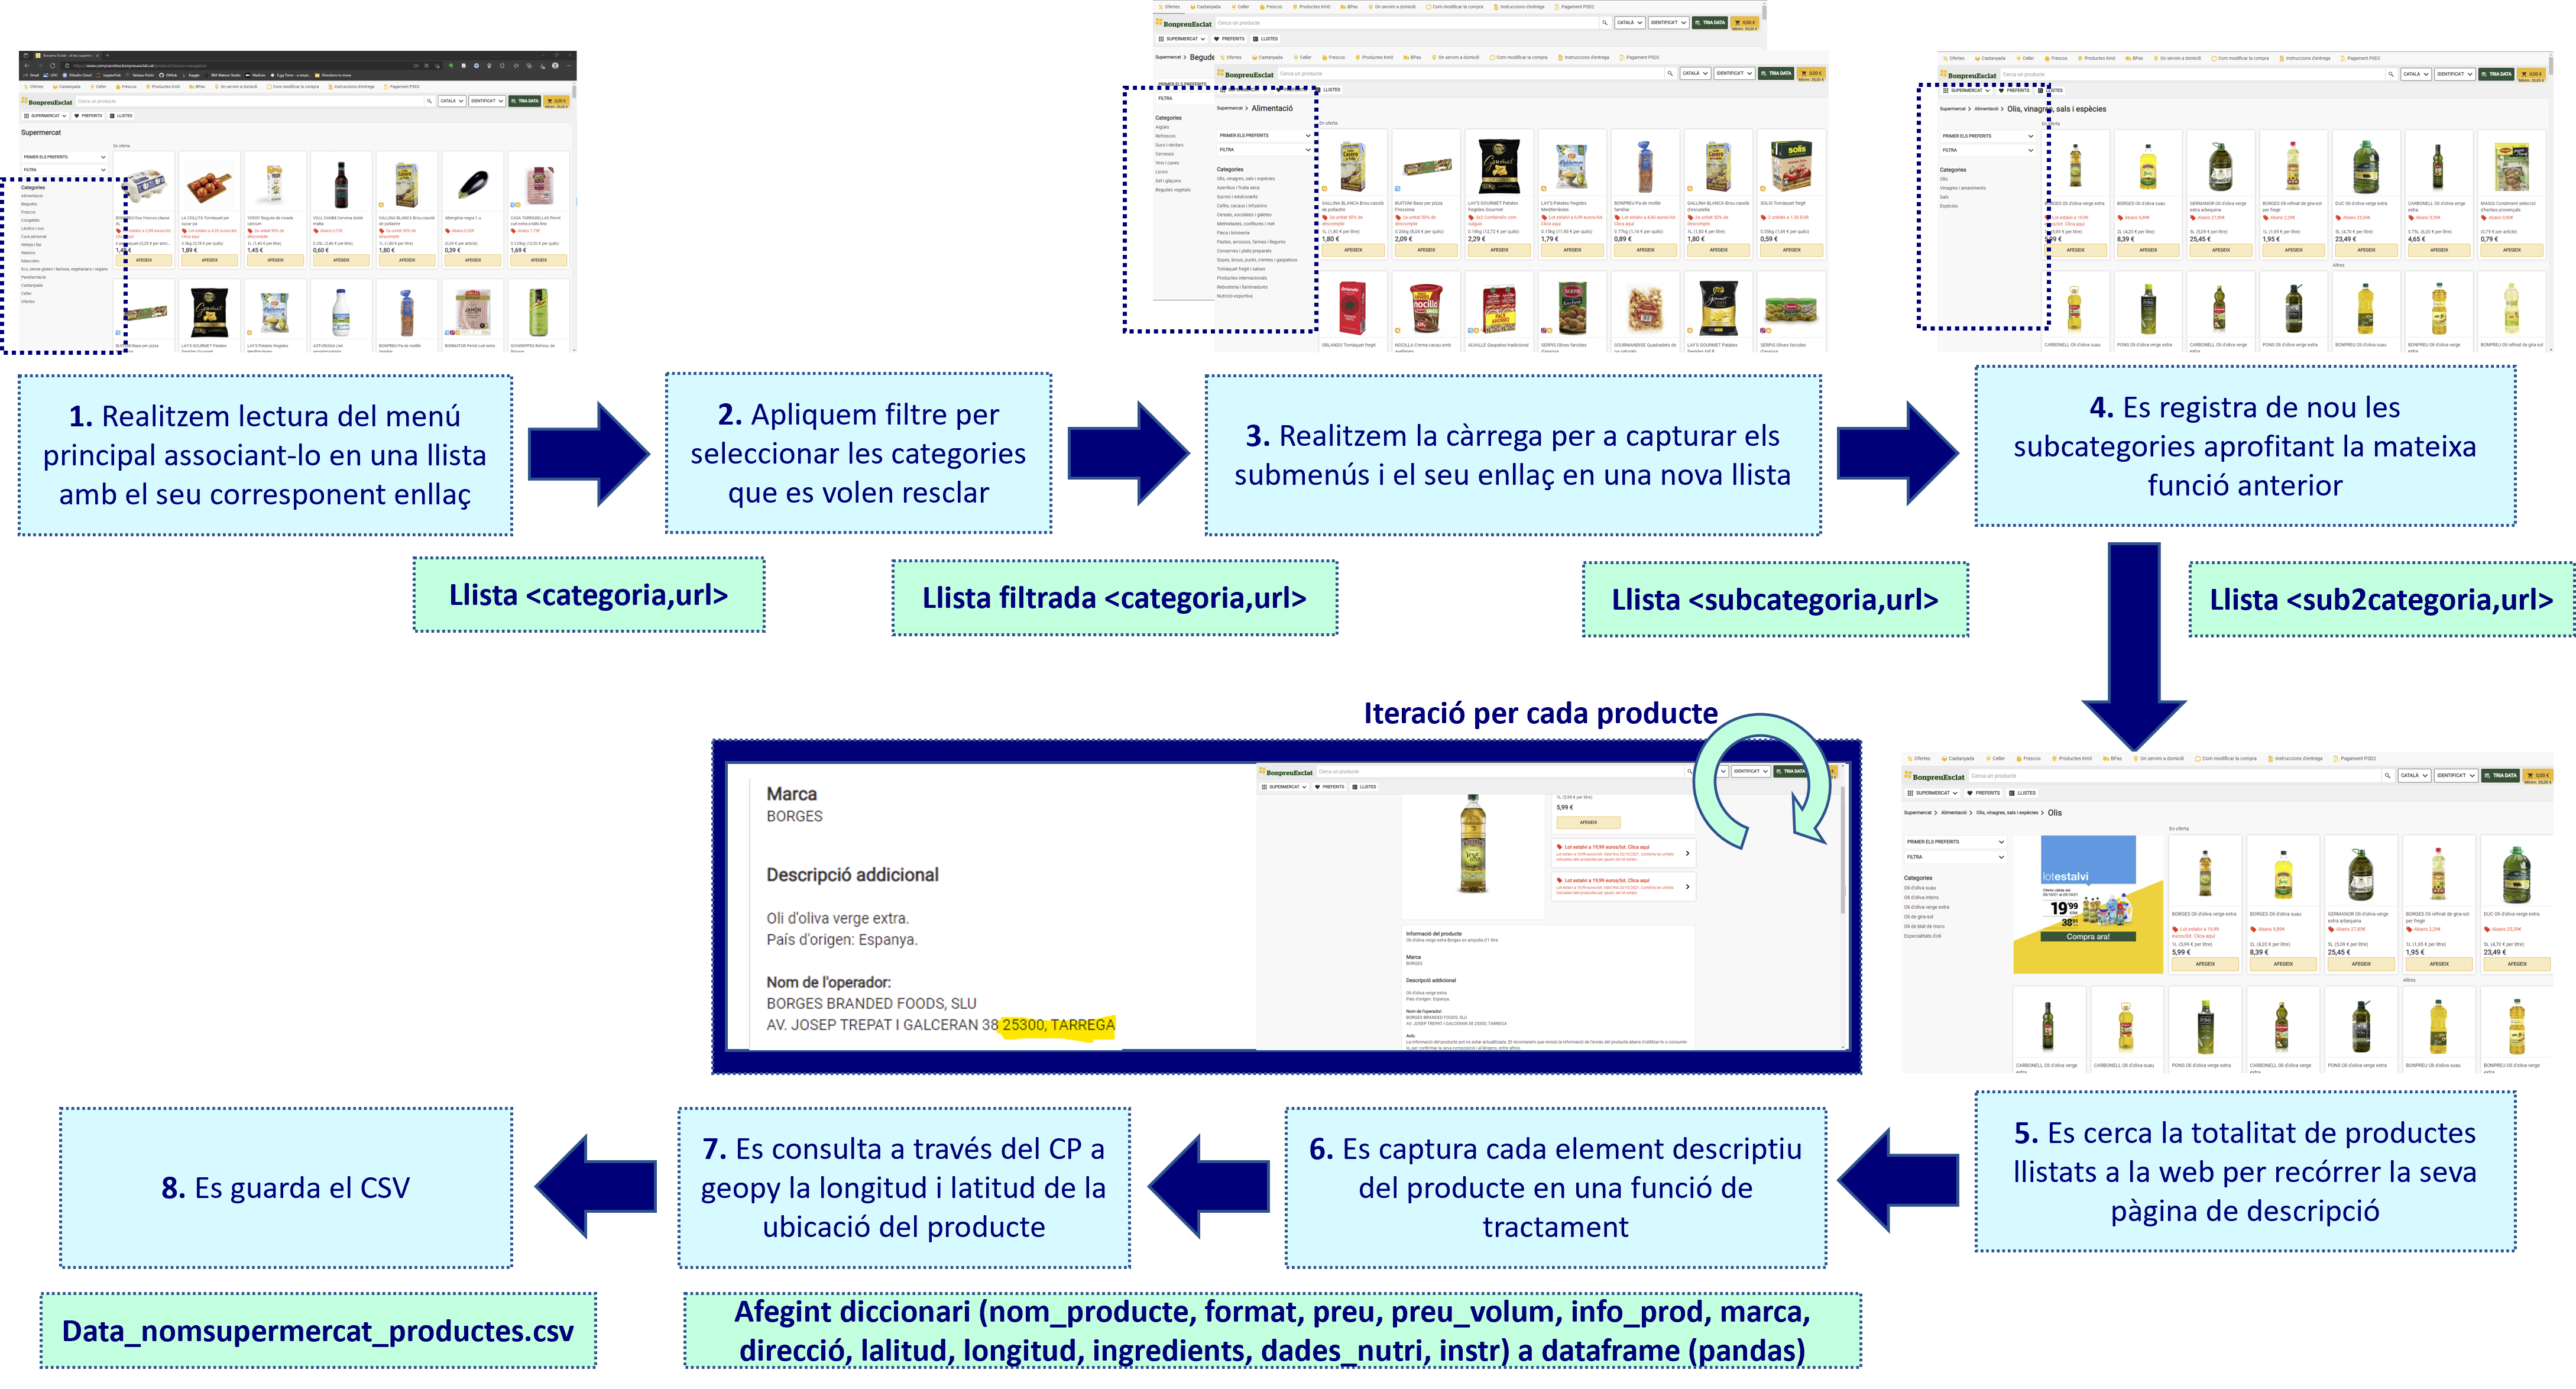
\includegraphics{../img/infographic_productesProximitatScraper_procediment}
	\caption{Procediment del funcionament del webscraper}
\end{figure}



\section{Contingut}
La taula següent presenta els camps del dataset.
\begin{table}[htbp]
	\centering
	\resizebox{17cm}{!} {
	\begin{tabular}{|l|l|}
		\hline
		\rowcolor[HTML]{000078} 
		\multicolumn{1}{|c|}{\cellcolor[HTML]{000078}{\color[HTML]{FFFFFF} \textbf{Camp}}} &
		\multicolumn{1}{c|}{\cellcolor[HTML]{000078}{\color[HTML]{FFFFFF} \textbf{Descripció}}} \\ \hline
		subcategoria       & Llista la categoria a la que pertany el producte, permeten relacionar productes similars. \\ \hline
		nom\_producte & Nom descriptiu intern de BonPreu que identifica el producte. \\ \hline
		format  & Format de l'envàs amb el que es presenta el producte \\ \hline
		preu       & Preu actual del producte \\ \hline
		preu\_volum & Preu per unitat de volum amb el que es presenta el producte. \\ \hline
		info\_prod  & Informació general del producte \\ \hline
		marca  & Empresa responsable del producte. \\ \hline
		direccio       & Direcció del producte. \\ \hline
		latitud & Distància angular mesurada sobre un meridià, entre una localització terrestre i l'Equador. \\ \hline
		longitud  &  Distància angular sobre un meridià, entre una localització terrestre i Greenwich.\\ \hline
		ingredients       & Components del producte separats per una coma (només aliments). \\ \hline
		dades\_nutri & Informació nutricional del producte (només aliments). \\ \hline
		instr  & Instruccions dels productes \\ \hline
	\end{tabular}
	}
	\caption{Definició dels camps dels que es composa el dataset.}
	\label{tab:Taula de contribucions}
\end{table}
\\\\Els nom del supermercat i la data de captació s'ha considerat que era millor incorporar-los al nom del fitxer per reduir el pes del fitxer amb informació repetida.

\section{Agraïments}
La font d'informació d'on s'han recollit les dades és la pàgina web de \url{https://www.compraonline.bonpreuesclat.cat/products?source=navigation} i la seva plataforma en línia.  
Per aconseguir les dades s'han emprat tècniques de \textit{Web Scraping} emprant el llenguatge Python i les llibreries Request i BeautifulSoup4. Per aconseguir els posicionament del producte (longituds i latituds), així com el càlcul en quilòmetres s'ha emprat la llibreria GeoPy.


\section{Inspiració}
Cada vegada que anem a comprar, no únicament estem escollint productes, sinó que els votem. Com a consumidors tenim la força de que els productes i les seves empreses productores persisteixin en el temps. Per tant, l'acció de comprar un producte suposa un impacte en la sostenibilitat socio-econòmica i en el medi ambient. Informar al consumidor de la distància del centre de producció pot despertar la consciència de reduir les  cadenes de subministrament i beneficiar la comunitat propera.
\\\\
Aquesta pràctica intenta treballar el punt 12 dels ODS, els 17 objectius de desenvolupament sostenible marcats per l'agenda 2030 de les Nacions Unides ((\url{http://www.globalgoals.org/}).
\\\\
Aquest punt parla de \textbf{garantir patrons de consum i producció sostenibles}, i afecta especialment en dos dels punts:
\begin{itemize}
	\item 12.1 Implementar el marc de consum i producció sostenibles en 10 anys
	\item 12.6 Animar les empreses a adoptar pràctiques sostenibles i informes de sostenibilitat
\end{itemize} 
\begin{figure}[htb]
	\centering
	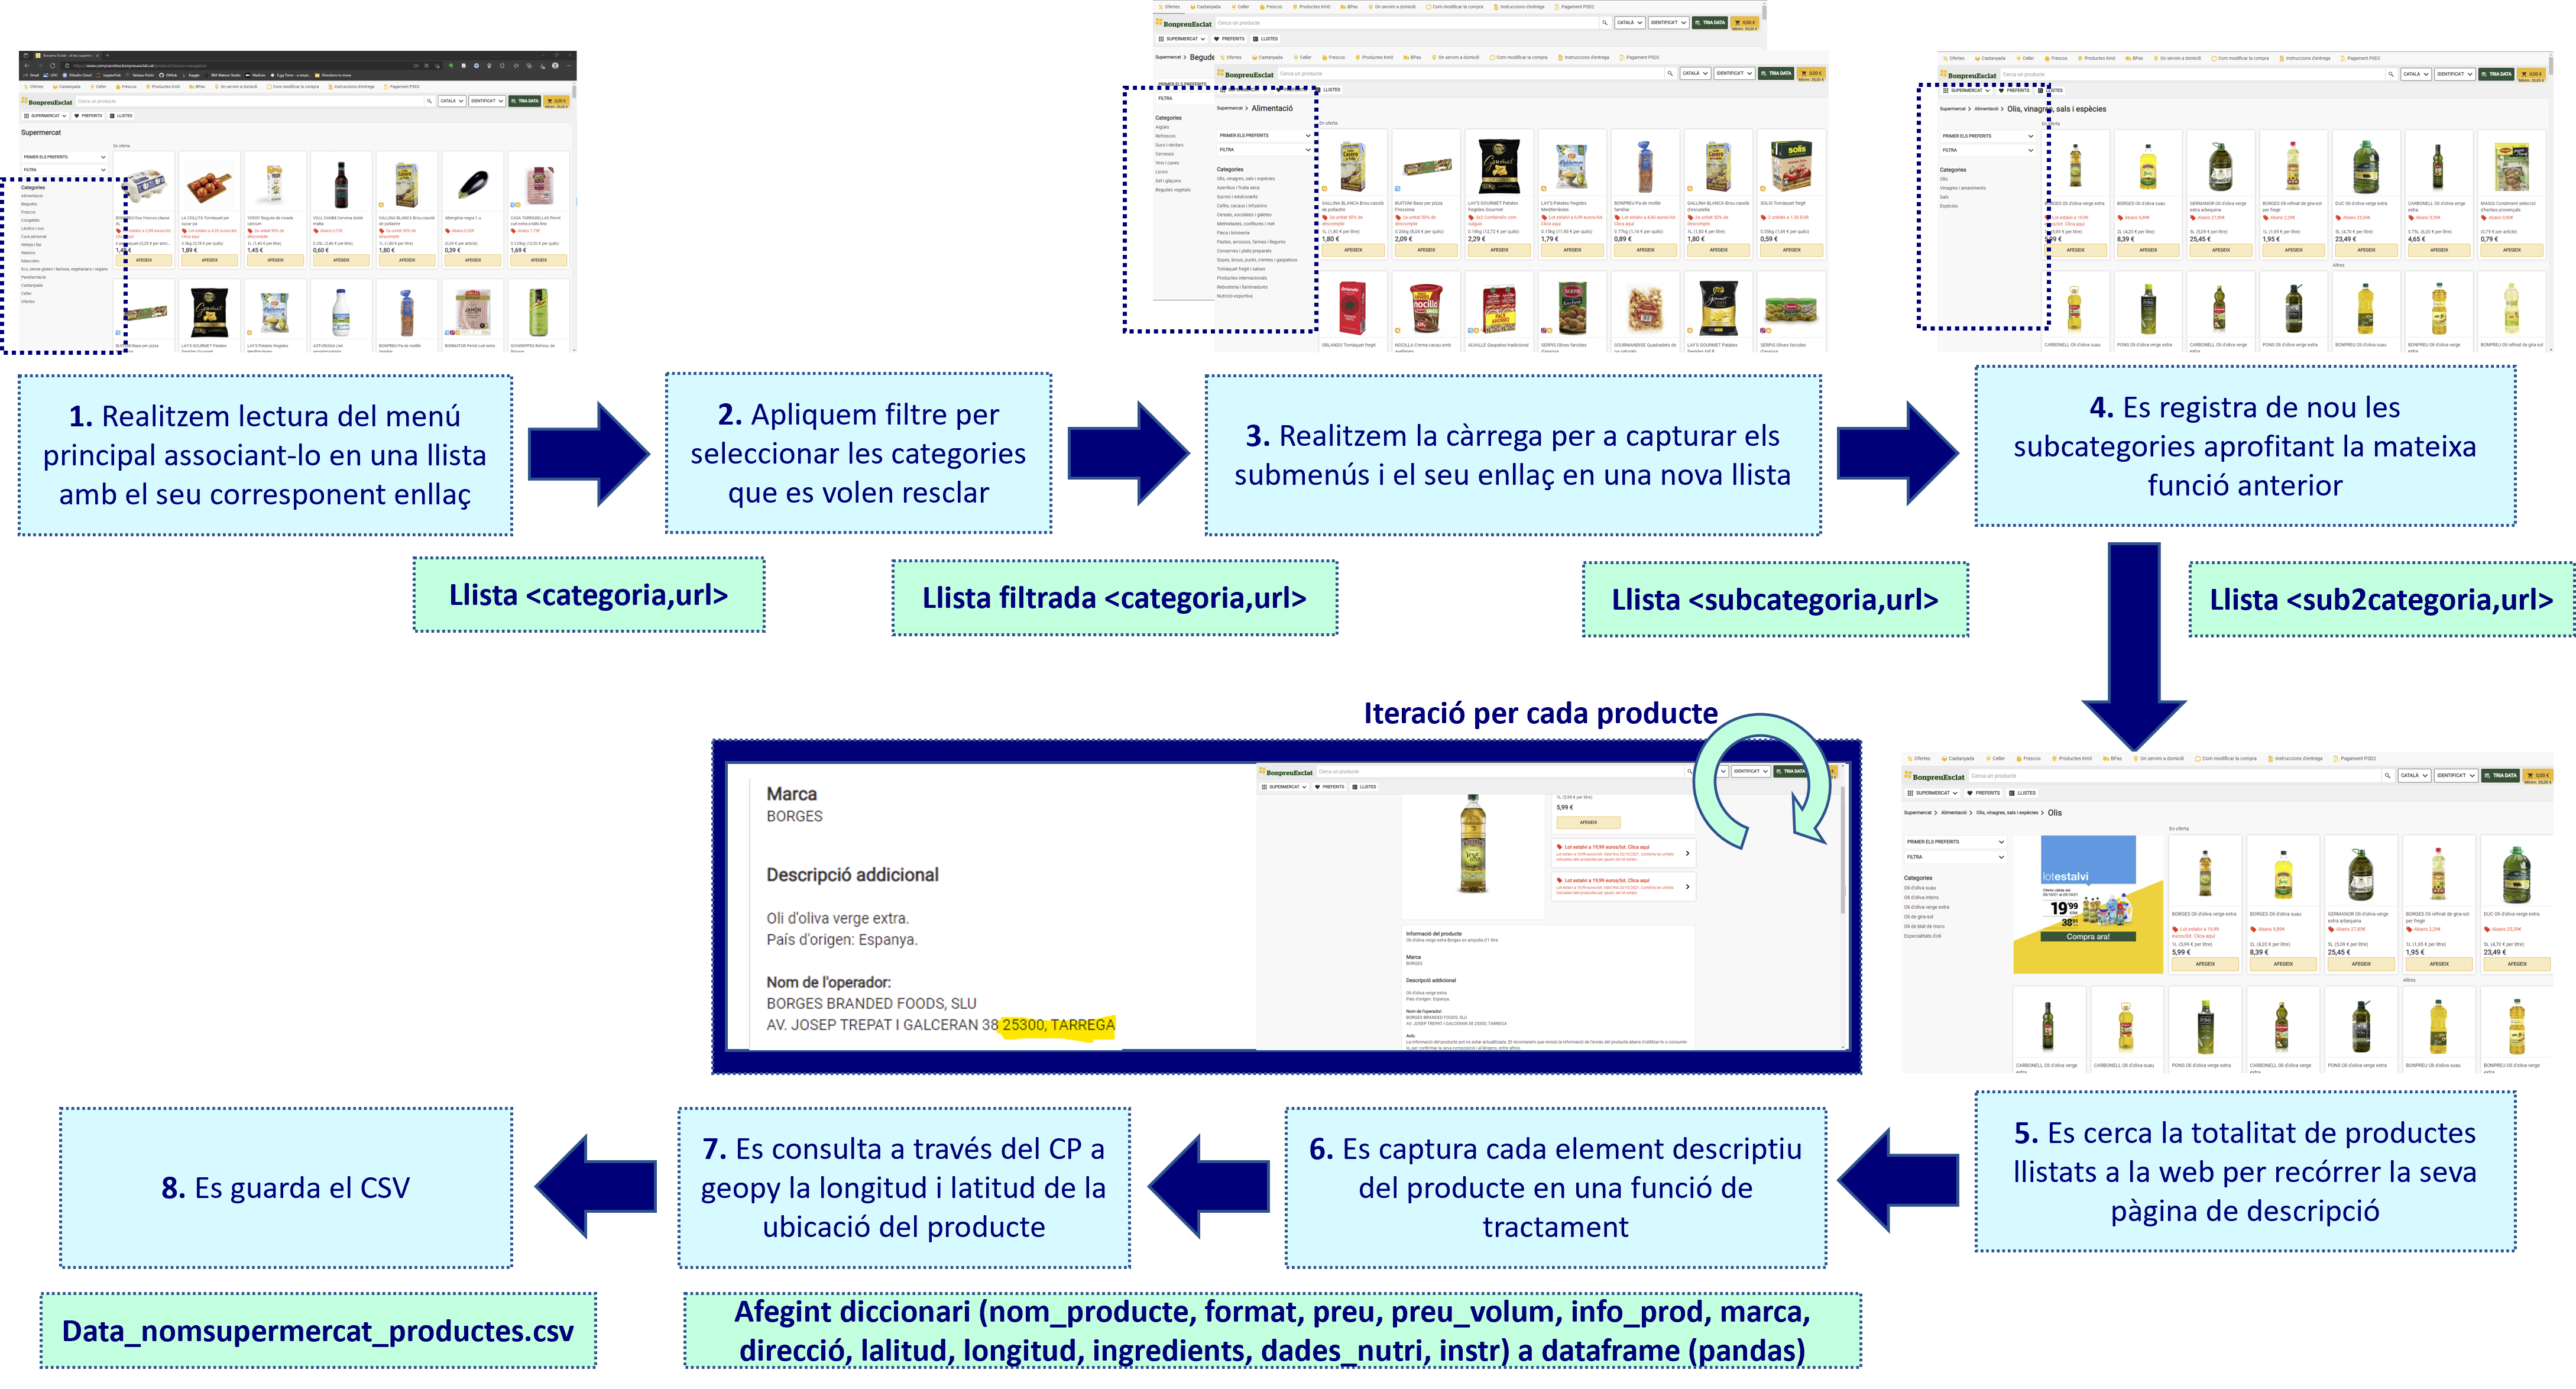
\includegraphics[width=0.7\textwidth]{../img/infographic_productesProximitatScraper_procediment}
	\caption{Captura dels 17 objectius de l'agenda 2030}
\end{figure}
Si en la llista de la compra s'indiqués la distància a la que es troba el centre productor de cada producte, es permetria entendre quins d'aquests recorren major distància. És a dir, ens permetria donar-nos compte de quins articles podríem canviar per alternatius més pròxims.
També ens permetria veure si hi ha algun producte sense productor pròxim en la nostra zona. Aquest podria ser un bon sistema per identificar possibilitats de negoci.
\\\\
Tot i aquest enfocament, la base de dades de producte s'ha estructurat per poder donar resposta a moltes més preguntes:
\begin{itemize}
	\item Seguiment de preus. Llançant el programa de forma cíclica es podria avaluar quina evolució de preu tenen els diversos productes. Pregunta: Quin és el millor dia del mes per anar a comprar? Per exemple, a través d'una rutina Cron en un sistema Linux corrent en una SBC com la Raspberry.
	\item Validar quins productes són els que ofereixen major oferta o nombre de productes
	\item Detectar quins productes no tenen marca blanca a través de validar subcategories i marques.
	\item Validar quin increment suposen els productes sense gluten davant de productes amb gluten. Quin percentatge de la compra suposen aquests articles especials?
	\item Comprovar quins aliments són els que disposen de major nombre de grasses saturades a través del camp de valors nutricionals. Quins són els aliments amb menors grasses saturades?
\end{itemize} 

\section{Llicència}

\section{Codi}
El codi font d'extracció i el dataset creat a tall d'exemple són accessibles a través de GitHub. Per a poder accedir al contingut pot visitar el següent enllaç:
\url{https://github.com/joanmorral/producteProximitatScrapper} 

El programa emprat per a la fase d'investigació a sigut jupyter notebook, ja que permet iterar amb dades descarregades.
Per a realitzar la codificació del programa final en format *.py s'ha emprat Pycharm, ja que es requeria un fitxer format *.py i  

\section{Dataset}


\section{Contribucions}
La taula de contribucions és la següent:
\\\\
\begin{table}[htbp]
	\centering
	\begin{tabular}{|l|l|}
		\hline
		\rowcolor[HTML]{000078} 
		\multicolumn{1}{|c|}{\cellcolor[HTML]{000078}{\color[HTML]{FFFFFF} \textbf{Contribucions}}} &
		\multicolumn{1}{c|}{\cellcolor[HTML]{000078}{\color[HTML]{FFFFFF} \textbf{Signatura}}} \\ \hline
		Investigació prèvia       & JMV, NGS \\ \hline
		Redacció de les respostes & JMV, NGS \\ \hline
		Desenvolupament del codi  & JMV, NGS \\ \hline
	\end{tabular}
	\caption{Contribucions en cada apartat.}
	\label{tab:Taula de contribucions}
\end{table}

\section{Recursos}

\end{document}
